\documentclass{beamer}

\usepackage{fix-cm}
\usepackage{soul}
\usepackage{float}
\usepackage{tikz}

\usepackage{color}
\definecolor{dblackcolor}{rgb}{0.0,0.0,0.0}
\definecolor{dbluecolor}{rgb}{.01,.02,0.7}
\definecolor{dredcolor}{rgb}{0.8,0,0}
\definecolor{dgraycolor}{rgb}{0.30,0.3,0.30}
\usepackage{listings}
\lstdefinelanguage{Sage}[]{Python}
{morekeywords={True,False,sage,singular},
sensitive=true}
\lstset{frame=none,
          showtabs=False,
          showspaces=False,
          showstringspaces=False,
          commentstyle={\ttfamily\color{dredcolor}},
          keywordstyle={\ttfamily\color{dbluecolor}\bfseries},
          stringstyle ={\ttfamily\color{dgraycolor}\bfseries},
          language = Sage,
          basicstyle={\scriptsize \ttfamily},
          aboveskip=.3em,
          belowskip=.1em
          }

\usepackage{fancybox}
\usepackage{graphicx}
\usepackage{amsmath}
\usepackage{amsfonts}
\usepackage{amssymb}
\usepackage{amsthm}
\usepackage{url}


\DeclareMathOperator{\Gap}{Gap}
\DeclareMathOperator{\Li}{Li}
\DeclareGraphicsRule{.tif}{png}{.png}{`convert #1 `dirname #1`/`basename #1 .tif`.png}

\newcommand{\mycaption}[1]{\begin{quote}{\bf Figure: } \large #1\end{quote}}

\newcommand{\ill}[3]{%
   \begin{figure}[H]%
   \vspace{-2ex}
   \centering%
   \includegraphics[width=#2\textwidth]{illustrations/#1}%
   \caption{#3}%
   \vspace{-2ex}
    \end{figure}}

\newcommand{\illtwo}[4]{%
   \begin{figure}[H]\centering%
   \includegraphics[width=#3\textwidth]{illustrations/#1}$\qquad$\includegraphics[width=#3\textwidth]{illustrations/#2}%
   \caption{#4}%
    \end{figure}}

\newcommand{\illthree}[5]{%
   \begin{figure}[H]%
\centering%
   \includegraphics[width=#4\textwidth]{illustrations/#1}$\qquad$\includegraphics[width=#4\textwidth]{illustrations/#2}$\qquad$\includegraphics[width=#4\textwidth]{illustrations/#3}%
   \caption{#5}%
    \end{figure}}




\def\GL{\mathrm{GL}}
\def\PGL{\mathrm{PGL}}
\def\PSL{\mathrm{PSL}}
\def\GSP{\mathrm{GSP}}
\def\Z{\mathrm{Z}}
\def\Q{\mathrm{Q}}
\def\Gal{\mathrm{Gal}}
\def\Hom{\mathrm{Hom}}
\def\Ind{\mathrm{Ind}}
\def\End{\mathrm{End}}
\def\Aut{\mathrm{Aut}}
\def\loc{\mathrm{loc}}
\def\glob{\mathrm{glob}}
\def\Kbar{{\bar K}}
\def\D{{\mathcal D}}
\def\L{{\mathcal L}}
\def\R{{\mathcal R}}
\def\G{{\mathcal G}}
\def\W{{\mathcal W}}
\def\H{{\mathcal H}}
\def\OH{{\mathcal OH}}



\newcommand{\RH}{Riemann Hypothesis\index{Riemann Hypothesis}}


\title{PRIMES}
\author{Barry Mazur}
\date{\today}

\begin{document}

\begin{frame}
\titlepage

{\it (A discussion of `Primes: What is Riemann's Hypothesis?,' the book I'm currently writing with William Stein)}
\end{frame}

\begin{frame}
\frametitle{William:}
 (Here I'll put the video)
\end{frame}
\begin{frame}

\frametitle{The impact of the Riemann Hypothesis}
\ill{sarnak}{0.20}{Peter Sarnak}

\begin{quote}
``The Riemann hypothesis is the central problem and it implies many,
many things. One thing that makes it rather unusual in mathematics
today is that there must be over five hundred papers---somebody should
go and count---which start `Assume the Riemann hypothesis,' and
the conclusion is fantastic. And those [conclusions] would then become
theorems ... With this one solution you would have proven five hundred
theorems or more at once.'' 
\end{quote}

\end{frame}
\begin{frame}
\frametitle{An expository challenge}
     The approach you take when you try to explain anything depends upon your intended audience(s).  In our case we wanted to reach two quite different kinds of readers (at the same time):
     \vskip20pt
     \begin{itemize} \item High School students who are already keen on mathematics,
        \vskip20pt
     \item A somewhat  older crowd of scientists (e.g., engineers)  who have a nonprofessional interest in mathematics.
     \end{itemize}
\end{frame}
\begin{frame}\frametitle{\bf\large What {\em sort} of Hypothesis is the \RH{}?}
 \begin{center}
       \shadowbox{ \begin{minipage}{0.91\textwidth}
\mbox{}       \vspace{0.2ex}
 
Consider the seemingly innocuous series of questions:

\begin{quote}
\begin{itemize}
\item How many primes  (2, 3, 5, 7, 11, 13, $\ldots$) are there less than 100?
\item How many less than 10,000?
\item How many less than 1,000,000?
\end{itemize}

More generally, how many primes are there less than any given number $X$?
\end{quote}

Riemann's Hypothesis tells us that a strikingly
simple-to-describe function is a ``very good approximation'' to the number of
primes less than a given number $X$. We now
see that if we could prove this {\em Hypothesis of Riemann} we would have
the key to a wealth of powerful mathematics. Mathematicians are eager
to find that key.


\vspace{1ex}
\end{minipage}}\end{center}
      \end{frame}
\begin{frame}\frametitle{An expository frame---and goal}\vskip10pt
\ill{raoulbott}{0.20}{Raoul Bott (1923--2005)\label{fig:bott}}

Raoul Bott, once
said---giving advice to some young mathematicians---that whenever one
reads a mathematics book or article, or goes to a math lecture, one
should aim to come home with something very specific (it can be small,
but should be {\em specific}) that has application to a wider class of
mathematical problem than was the focus of the text or lecture. 

\end{frame}

\begin{frame}\frametitle{Setting the frame}
 If we
were to suggest some possible {\em specific} items to come home with,
after reading our book, three key phrases -- {\bf prime numbers}, {\bf
  square-root accurate}, and {\bf spectrum} -- would head the
list.

\end{frame}

\begin{frame}\frametitle{PRIMES: order appearing random }
\vskip10pt
\ill{zagier}{.15}{Don Zagier}


\begin{quote}

``{\bf [Primes]}
\begin{itemize}\item are the most arbitrary and ornery objects studied by mathematicians:
  they grow like weeds among the natural numbers, seeming to obey no
  other law than that of chance, and nobody can predict where the next
  one will sprout. \item  exhibit stunning
  regularity $\dots$
  they obey their laws with almost military precision.''\end{itemize}
\end{quote}
\end{frame}

\begin{frame}\frametitle{How to nudge readers to feel the orneriness of primes }

 There is something compelling about `physically' hunting for a species of  mathematical object, and collecting specimens of it. Our book emphasizes this approach for our readers. Here are some routes that allow you to 'pan' (in different ways)  for  primes:

\vskip20pt


\centerline{ {\bf Factor trees}  and {\bf Sieves}}


\vskip10pt


\centerline{and}


\vskip10pt


\centerline{\bf Euclid's Proof of the Infinitude of Primes.}
\end{frame}

\begin{frame}\frametitle{\bf Factor trees}

\illtwo{factor_tree_300_a}{factor_tree_300_b}{.47}


\end{frame}

\begin{frame}\frametitle{\bf Sieves}
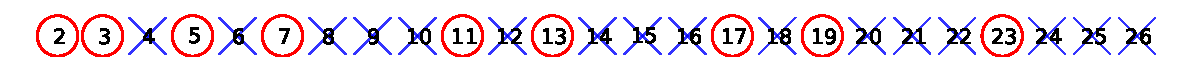
\includegraphics[width=\textwidth]{illustrations/circled_primes}
\end{frame}

\begin{frame}\frametitle{\bf The ubiquity of primes}
\vskip10pt
\ill{dulcinea1}{.2}{Don Quixote and ``his'' Dulcinea del Toboso}
\vskip10pt
Numbers are obstreperous things. Don Quixote encountered this when he
requested that the ``bachelor'' compose a poem to his lady Dulcinea del
Toboso, the first letters of each line spelling out her name.
\end{frame}

\begin{frame}\frametitle{\bf The stubbornness of primes and knights}
The
``bachelor'' found
\vskip10pt

\begin{quote}
  ``a great difficulty in their composition because the number of
  letters in her name was $17$, and if he made four Castilian stanzas
  of four octosyllabic lines each, there would be one letter too many,
  and if he made the stanzas of five octosyllabic lines each, the ones
  called {\em d{\'e}cimas} or {\em redondillas,} there would be three
  letters too few...'' 
\end{quote}

``It must fit in, however, you do it,'' pleaded Quixote, not willing to
grant the imperviousness of the number $17$ to division.
\end{frame}


\begin{frame}\frametitle{\bf Gaps: an example of a `question anyone might ask'}
\vskip10pt

\ill{zhang}{0.15}{Yitang Zhang\label{fig:zhang}}

{\Huge
In celebration of Yitang Zhang's recent result, consider the {\em gaps} between one prime and the next.}
\end{frame}\begin{frame}\frametitle{\bf Twin Primes}
{\Huge
\begin{quote} As of 2014, the largest known twin primes are  \vskip10pt
$$3756801695685\cdot 2^{666669} \pm 1$$ \vskip10pt
These enormous primes have $200700$ digits each.
\end{quote}}
\end{frame}
\begin{frame}\frametitle{\bf Gaps of width $k$}
Define
{\Huge $$
  \Gap_{k}(X)
$$
to be the number of pairs of {\em consecutive} primes $(p,q)$ with
$q<X$ that have ``gap $k$'' (i.e., such that their difference $q-p$ is
$k$). 

\vskip20pt

{\bf NOTE:} $\Gap_{4}(10)=0$ because despite $3$ and $7$ being separated
by $4$, they are not consecutive primes.}\end{frame}
\begin{frame}\frametitle{\bf Gap statistics}


\begin{table}[H]\centering
\caption{Values of $\Gap_{k}(X)$ \label{tab:gap}}
\vspace{1em}

{\small
\begin{tabular}{|l|c|c|c|c|c|c|}\hline
$X$ & $\Gap_{2}(X)$ & $\Gap_{4}(X)$& $\Gap_{6}(X)$ & $\Gap_{8}(X)$ &
 $\Gap_{100}(X)$ &   $\Gap_{252}(X)$\\\hline

$10$ & 2 & 0 & 0 & 0 & 0 & 0\\\hline
$10^{2}$ & 8 & 7 & 7 & 1 & 0 & 0\\\hline
$10^{3}$ & 35 & 40 & 44 & 15 & 0 & 0\\\hline
$10^{4}$ & 205 & 202 & 299 & 101 & 0 & 0\\\hline
$10^{5}$ & 1224 & 1215 & 1940 & 773 & 0 & 0\\\hline
$10^{6}$ & 8169 & 8143 & 13549 & 5569 & 2 & 0\\\hline
$10^{7}$ & 58980 & 58621 & 99987 & 42352 & 36 & 0\\\hline
$10^{8}$ & 440312 & 440257 & 768752 & 334180 & 878 & 0\\\hline

\end{tabular}
}
\end{table}
\end{frame}


\begin{frame}\frametitle{\bf How many primes are there?}
\vskip20pt

{\Huge $\pi(X):=$ \# of primes  $\le X$}
\vskip10pt

\ill{prime_pi_25_aspect1}{.8}{Staircase of primes up to 25\label{fig:staircase25}}\end{frame}
\begin{frame}\frametitle{\bf How many primes are there?}
\vskip20pt
\ill{prime_pi_100_aspect1}{.8}{Staircase of primes up to 100\label{fig:staircase100a}}

\end{frame}


\begin{frame}\frametitle{\bf Prime numbers viewed from a distance}
\vskip10pt
 {\Huge{\it Pictures of data magically become smooth curves as you telescope to greater and greater ranges.}}
\vskip20pt


\illtwo{prime_pi_1000}{prime_pi_10000}{0.4}{Staircases of primes up to 1,000 and 10,000\label{fig:staircases2}}
\end{frame}


\begin{frame}\frametitle{\bf Proportion of Primes}\vskip10pt
\ill{proportion_primes_100}{1}{Graph of the proportion of primes up to $X$ for each integer $X\leq 100$}
\end{frame}


\begin{frame}\frametitle{\bf Proportion of Primes at greater distance}\vskip10pt

\illtwo{proportion_primes_1000}{proportion_primes_10000}{0.46}{Proportion of primes for $X$ up to $1{,}000$ (left) and $10{,}000$ (right)}
\end{frame}




\begin{frame}\frametitle{\bf Gauss}\vskip10pt

\ill{gauss_tables_half}{.9}{A Letter of Gauss\label{fig:gauss_letter}}\end{frame}

\begin{frame}\frametitle{\bf Gauss' guess}\vskip10pt

{\Huge The `probability' that a number $N$ is a prime  is proportional to the reciprocal of its number of digits; more precisely the probability is
\vskip10pt $$1/\log(N).$$}\end{frame}

\begin{frame} 

{\Huge This would lead us to this guess for the approximate value of $\pi(X)$: \vskip10pt
  $$\Li(X):=\ \ \ \int_2^XdX/\log(X).$$}\end{frame}

\begin{frame}\frametitle{\bf Approximating $\pi(X)$}\vskip10pt



\ill{three_plots}{1.0}{Plots of $\Li(X)$ (top), $\pi(X)$ (in the middle), and $X/\log(X)$ (bottom).\label{fig:threeplots}}\end{frame}

\begin{frame}\frametitle{\bf The Prime Number Theorem}\vskip10pt
\ill{three_plots}{0.5}{Plots of $\Li(X)$ (top), $\pi(X)$ (in the middle), and $X/\log(X)$ (bottom).\label{fig:threeplots}}\vskip10pt

{\Huge All three graphs  {\it tend to $\infty$} at the same rate.}\end{frame}
\begin{frame}\frametitle{\bf Ratios versus Differences}
\vskip10pt
{\Huge \centerline{\bf PNT:}\vskip10pt  Ratios  ${\frac{\pi(X)}{Li(X)}}$ and ${\frac{\pi(X)}{X/\log(X))}}$\vskip10pt  tend to $1$ as $X$ goes to $\infty$.} 
\vskip10pt

{\Huge Much subtler question: what about their differences?

$$|\Li(X)-pi(X|?$$}\end{frame}

\begin{frame}\frametitle{\bf Riemann's
Hypothesis}

      \begin{center}
       \shadowbox{ \begin{minipage}{0.9\textwidth}
\mbox{}       \vspace{0.2ex}
       \begin{center}{\bf\large The {\bf \RH{}} (first formulation)}\end{center}
       \medskip

For any real number $X$ the number of prime numbers less than $X$ is
approximately $\Li(X)$ and this approximation is essentially square
root accurate.

\vspace{1ex}
\end{minipage}}
      \end{center}
\end{frame}
\end{document}
There are 455,052,512 primes less than ten billion; i.e.,
10,000,000,000 (so we might say that the chances are down to roughly
$1$ in $22$).

Primes, then, seem to be thinning out.  We return to the sifting process
we carried out earlier, and take a look at a few graphs, to get a sense of why
that might be so. There are a $100$ numbers less than or equal to
$100$, a thousand numbers less than or equal to $1000$, etc.: the
shaded graph in Figure~\ref{fig:sieve_2_100} that looks like a regular staircase, each step the
same length as each riser, climbing up at, so to speak, a 45 degree
angle, counts all numbers up to and including~$X$.

Fol






\end{document}
 The recent results of Zhang as sharpened by Maynard (and others) we mentioned above tell us that for  at least one even number $k$ among the  even numbers $k \le 252$,    $\Gap_{k}(X)$ goes to infinity as $X$ goes to infinity. One expects that this happens for {\it all} even numbers $k$. We expect this as well, of course, for $\Gap_{252}(X)$ despite what might be misconstrued as discouragement by the above data.

\ill{primegapdist}{1}{Frequency histogram showing the distribution of
  prime gaps of size $\leq 50$ for all primes up to $10^7$.  Six is
  the most popular gap in this data.  The vertical axis labels
  such as ``6e4'' mean $6\cdot 10^4=60{,}000$.
\label{fig:primegapdist}}


\ill{primegap_race}{1}{Plots of $\Gap_k(X)$ for $k=2,4,6,8$.  Which wins?}

Here is yet another question that deals with the spacing of prime
numbers that we do not know the answer to:

{\em Racing Gap $2$,  Gap $4$, Gap $6$, and Gap $8$ against each other:}

\begin{quote}
  Challenge: As $X$ tends to infinity which of $\Gap_2(X)$,
  $\Gap_4(X)$,
  $\Gap_6(X),$ or $\Gap_8(X)$ do you think will grow faster? How
  much would you bet on the truth of your guess? \bibnote{%
    Hardy and Littlewood give a nice conjectural answer to such
    questions about gaps between primes.  See Problem {\bf A8} of
    Guy's book {\em Unsolved Problems in Number Theory} (2004).
Note that Guy's book discusses counting the number $P_k(X)$ of pairs of
primes up to $X$ that differ by a fixed even number $k$; we have
$P_k(X)\geq \Gap_k(X)$, since for $P_k(X)$ there is no requirement
that the pairs of primes be consecutive.}
\end{quote}


\end{document}
%sagemathcloud={"zoom_width":90}